\chapter{Teori}
\paragraph{} Dette kapittelet vil gå dypere inn på den teoretiske delen rundt selve oppgaven. Her beskrives de grunnleggende elementene som benyttes i prosjektet, hva de betyr og hvordan de fungerer. I tillegg blir ulik terminologi som benyttes i rapporten forklart her og det er dermed nødvendig å lese og forstå denne delen før en fortsetter med å lese rapporten. Med dette ønsker gruppen å øke forståelsen til leseren og danne et bedre grunnlag for de som leser rapporten. Dette vil hjelpe med å velge den beste løsningen for bedriften.
\section{Grunnleggende elementer}
\paragraph{Hva er en server?} 
En server er et datamaskinprogram som forsørger forskjellige tjenester til forskjellige programmer og deres brukere. Datamaskinen serverprogrammet kjører på refereres til som en “server”. Servere deles ofte inn i forskjellige kategorier basert på hvordan de brukes, f.eks. en “Web Server” \footnote{http://whatis.techtarget.com/definition/server}

\paragraph{Hva er en nettsky?}  

En fremtidsrettet teknologi hvor data og informasjon lagres på servere som ligger på eksterne steder som er tilknyttet internett Nettskyen tillater brukere å lagre informasjon uten å behøve å selv drifte en egen server. Microsoft, Google, og Amazon. Nettskybasert databehandling tilbyr en rekke fordeler for fortetninger og brukere. Vi kan dele fordelene inn i 3 forskjellige grupperinger.\footnote{https://no.wikipedia.org/wiki/Nettskyen}.

\paragraph{Hva er en hybridløsning?} 

En hybrid-løsning i prosjektet handler om å finne en mulig vei for bedriften med blandede løsninger som kan være aktuelt å bruke. For eksempel, å bruke både interne servere som blir plassert hos bedriften og en liten cloud-løsning som befinner seg hos en annen leverandør.
Dette er noe som kan være aktuelt hvis bedriften ønsker å ha noe av dataene sine på huset.\footnote{http://www.dummies.com/programming/cloud-computing/hybrid-cloud/what-is-hybrid-cloud-computing/}

\paragraph{} Nettskyen, skyen eller cloud er en fellesbetegnelse på alt fra dataprosessering og datalagring til programvare på eksterne servere tilknyttet Internett. (En server er en programvare som tilbyr en eller flere tjenester over et datanettverk. Begrepet server, eller tjener på norsk er også ofte brukt på maskinvaren som programmet/programmene kjøres fra, så lenge maskinen har kapasiteten til å utføre oppgavene.

Vi kan også dele skytjenestene opp i forskjellige leveransemodeller. Da går det altså hovedsakelig ut på allmenn tilgjengelig {\small (Public Cloud)}, privat tilgjengelig {\small (Private Cloud)} og sist hybridsky {\small (Hybrid Cloud)};\par
\begin{description}[noitemsep]
\item[Public Cloud] En allmenn tilgjengelig sky betyr at skytjeneste er gjort tilgjengelig for alle kunder av leverandøren.
\item[Private Cloud] Privat tilgjengelig sky betyr at skytjenesten er gjort privat, og dedikert kun til en gruppe av kunder. Skytjenesten gjelder altså kun for virksomheten den er dedikert til. Som vi ser, her vil skyen typisk bli dedikert til den enkelte kunden eller den definerte kundegruppen. Denne løsningen åpner for en større grad av spesifikke tilpasninger.
\item[Hybrid Cloud] Hybrid sky er altså en blanding av tjenestene som kan leveres ovenfor. En god blanding av de begge.
\end{description}
\begin{figure}[H]
\centering
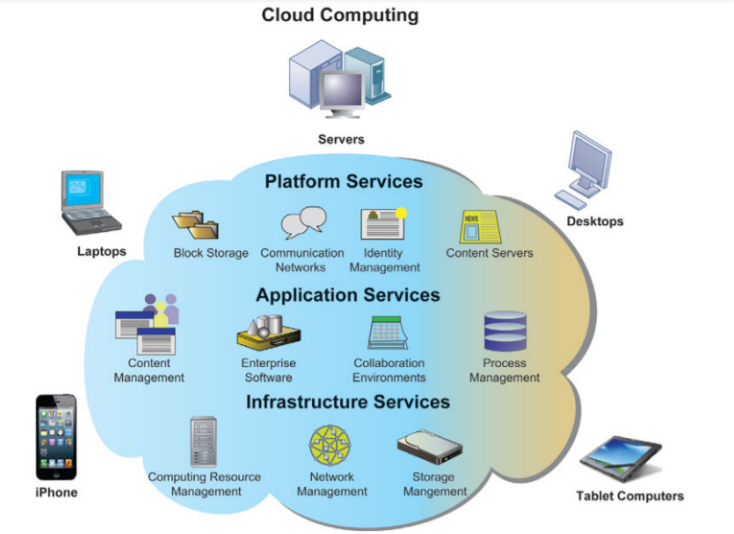
\includegraphics[width=6.5in]{Bilder/cc.PNG}
\caption{En visuell representasjon av hvordan Sky tjenester er satt opp.(Laudon \& Laudon, 2016, s.223)}
\end{figure}

Som vi kan lese ovenfor, tilbyr skybaserte løsninger en rekke forskjellige modeller. Disse modellene er veldig fleksible, brukervennlige og tilpasset behov. Under vil du finne ulike skytjenester som tilbys fra bedrifter som Microsoft, Amazon og Google:
\begin{description}
\item Microsoft Azure er en skytjeneste som er utviklet av Microsoft og som tilbyr brukere av tjenesten en rekke verktøy og programmer knyttet til lagring, utvikling og distribuering av informasjon og data.\footnote{https://azure.microsoft.com/nb-no/}

\item Amazon Web Services (AWS) er Amazon sitt svar på en skytjeneste. Med Amazon AWS har man tilgang til en rekke funksjoner, deriblant muligheten til å enkelt lagre store og små datamengder, levere ulikt innhold til brukere og kraftige maskiner som tar seg av mye av arbeidet.\footnote{https://aws.amazon.com/about-aws/}

\item Google Disk er en versjon av en Sky tjeneste forenklet så mye som mulig for å tilpasse så mange brukere som mulig. Med Google Disk har man tilgang til alle filene og mappene sine, uansett hvor man er, med et svært enkelt brukergrensesnitt og hvor mye av de administrative oppgavene blir tatt hånd om.\footnote{https://www.google.com/drive/}

\item Microsoft PowerShell er et komandolinjeskall for systemadministratorer. PowerShell fungerer i form av at systemadministrator skriver inn kommando for å styre operativsystemet til å utføre bestemte oppgaver. Det å arbeide i PowerShell kan få brukeren til å styre programmer og manipulerer elementer i systemets database. Når det er nevnt kreves det noe datakunnskaper for å utføre disse manipulasjonene. \footnote{http://www.datamaskin.biz/Systems/windows/212342.html}
\end{description}

\section{Server}
\paragraph{} En server er et datamaskinprogram som forsørger forskjellige tjenester til forskjellige programmer og deres brukere. Datamaskinen serverprogrammet kjører på refereres til som en “server”. Servere deles ofte inn i forskjellige kategorier basert på hvordan de brukes, f.eks. en “Web Server” \todo[author=Ole]{{\scriptsize Bruk heller enquotes}} 
\begin{figure}[H]
\centering
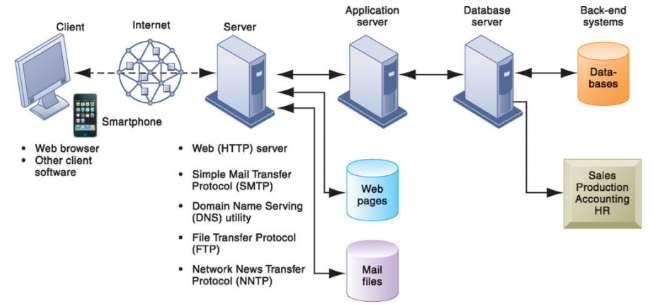
\includegraphics[width=6.5in]{Bilder/cc2.PNG}
\caption{En modell som viser en visuell forklaring på hvordan datamaskiner, Internet og servere henger sammen med andre systemer. (Laudon \& Laudon, 2016, s.305) }
%\todo[inline,author=Ole]{{\scriptsize Dere må ref'e til hvor dette bildet er tatt fra. Ved å linke til bibliografien deres. Dette må dere gjøre med ALLE bilder og grafikk dere har hentet fra andre kilder en dere selv. Dette gjør dere ved å bruke \textbackslash cite\{labeltype:refname\}}}
\end{figure}

\section{Terminologi}
\paragraph{} {\bfseries Interne servere:} Interne servere i en bedrift vil si at serveren står fysisk i lokalene til selskapet. Disse serveren vil altså lagre data, kjøre applikasjoner og holde på forskjellige API/ERP løsninger som selskapet benytter. \footnote{https://no.wikipedia.org/wiki/Server}
\footnote{http://whatis.techtarget.com/definition/server}

\paragraph{} {\bfseries ERP:} Enterprise resource planning (ERP) er en programvare som støtter flere av en bedrifts virksomgetsområder,  som produksjon, lager, salg , innkjøp og økonomi.  Målet med ERP er å håndtere virksomgetens informasjon.
\footnote{https://www.oracle.com/applications/erp/what-is-erp.html}

\paragraph{} {\bfseries Operativsystem:} Et operativsystem (OS) er den grunnleggende programvaren på en datamaskin, og det som tildeler de forskjellige ressursene i datamaskinen til andre programmer.
\footnote{https://no.wikipedia.org/wiki/Operativsystem}

\paragraph{} {\bfseries PaaS(Platform as a service):}  Plattform som en tjeneste eller applikasjonsplattform som en tjeneste (aPaaS) er en kategori av cloud 
computing-tjenester som gir en plattform som gjør det mulig for kunder å utvikle, kjøre og administrere applikasjoner 
uten kompleksiteten i å bygge og vedlikeholde infrastrukturen som vanligvis er knyttet til å utvikle Og lanserer en app.
\footnote{https://en.wikipedia.org/wiki/Platform\_as\_a\_service}

\paragraph{} {\bfseries IaaS(Infrastructure as a Service):} Infrastruktur som en tjeneste er en form for cloud computing som gir databehandlings ressurser over Internett.
\footnote{http://searchcloudcomputing.techtarget.com/definition/Infrastructure-as-a-Service-IaaS}

\paragraph{} {\bfseries SaaS(Software as a Service):} Programvare som en tjeneste er en programvaredistribusjonsmodell 
der en tredjepartsleverandør er vert for programmer og gjør dem tilgjengelige for kunder over Internett.
\footnote{http://searchcloudcomputing.techtarget.com/definition/Software-as-a-Service}

\paragraph{} {\bfseries Data:} Informasjon, brukes for grunnlag av begrynnelse, diskusjon eller beregninger. 
\footnote{https://www.merriam-webster.com/dictionary/data}

\paragraph{} {\bfseries API:} Application Programming Interface, er et programfunksjon som lar brukeren koble sammen flere programmer.  Man kan da utveksle informasjon på tvers av programmene. 
\footnote{}
\paragraph{} {\bfseries Programvare:} Programvare (engelsk: software) er en fellesbetegnelse på dataprogrammer. Alt som er digitalt i dag har en form for programvare. 
\footnote{http://www.computerhope.com/jargon/s/software.htm}

\paragraph{} {\bfseries Maskinvare:} Maskinvare er de fysiske delene en server/datamaskin består av.
\footnote{http://www.computerhope.com/jargon/h/hardware.htm}
\footnote{http://www.computerhope.com/issues/ch000039.htm}

\paragraph{} {\bfseries Skytjenste (Cloud):} En Skytjeneste (Cloud) er et sett med applikasjoner, tjenester, lagring og maskinvare som opprettholdes og driftes av en tredje-part, som tillater andre bedrifter og organisasjoner å enkelt kunne lagre data og informasjon, uten å måtte bry seg om det tunge, administrative arbeidet som må gjøres for å drifte en slik løsning. Skytjenestene tillater brukere å lagre informasjon og data på en server som befinner seg på et eksternt sted på internett for å gjøre det så enkelt som mulig for brukeren.
\footnote{https://www.datatilsynet.no/Teknologi/Skytjenester---Cloud-Computing/Hva-er-nettskytjenester/}
\footnote{https://www.anskaffelser.no/it/temaer-it/skytjenester-cloud}

\paragraph{} {\bfseries Hybrid Cloud:} En "Hybrid Cloud" eller en hybrid skytjeneste, er en form for Skytjeneste som kombinerer og blander tjenestene og egenskapene fra de grunnleggende formene for nettskyer, Public og Private cloud og tilbyr brukerne å benytte seg av en blanding av disse for å oppnå et enhetlig, sikkert og automatisert lagrings system for både viktig og mindre viktig data og informasjon innenfor bedriften.
\footnote{https://www.microsoft.com/nb-no/cloud-platform/hybrid-cloud}

\paragraph{} {\bfseries SSD:} Solid State Drive (SSD) er en nyere form for harddisk (maskinvare) som benyttes som et lagringsmedium hvor søketiden og lagringen foregår med høyere hastighet enn med en vanlig harddisk. Som følge av den kjappere lagringen som en SSD kan gjennomføre, koster også disse harddiskene mer enn de vanlige harddiskene.
\footnote{https://www.komplett.no/category/10088/datautstyr/lagring/harddisker/ssd}
\footnote{http://uk.pcmag.com/storage-devices-reviews/8061/feature/ssd-vs-hdd-whats-the-difference}

\paragraph{} {\bfseries HDD:} Hard Disk Drive (HDD) er den tradisjonelle formen for en harddisk og er et lagringsmedium som er tilstrekkelig brukt i verden. Slike tradisjonelle harddisker har ofte en rekke ulemper ved seg, blant annet at de er sårbare og ikke minst tregere med å gjennomføre lagring enn nyere harddisker.
\footnote{http://uk.pcmag.com/storage-devices-reviews/8061/feature/ssd-vs-hdd-whats-the-difference}


\paragraph{} {\bfseries iSCSI:} Internet Small Computer Systems Interface (iSCSI) er en internet protokoll som står for den lagringen som gjennomføres over internett. iSCSI håndterer lagringen av data over internett, hvor det ikke er noen begrensning på avstander. Store organisasjoner benytter seg av denne protokollen hvor de tar imot informasjon og data fra andre brukere og lagrer disse i store datasentre. Kundene kan dermed gjennomføre lagring uten behov for fysiske harddisker.
\footnote{https://no.wikipedia.org/wiki/ISCSI}

\paragraph{} {\bfseries DDOS-angrep:} Et DDOS-angrep (distribuert tjenestenekt) er en form for Internett angrep hvor maskinene til et offer angripes og hvor brukeren, som blir angrepet, hindres i å gjennomføre handlinger eller få tilgang til informasjon. Dette kjennetegnes ofte ved man mister Internet tilgang. Dette kan føre til stor nedetid og koste dyrt for de som angripes.
\footnote{http://www.digitalattackmap.com/understanding-ddos/}
\footnote{https://no.wikipedia.org/wiki/Tjenestenektangrep}

\paragraph{} {\bfseries Ulovlig Hacking:} Ulovlig Hacking er en form for datakriminalitet hvor en person benytter sine ferdigheter, programmer og løsninger for å bryte seg inn og ulovlig hente informasjon eller manipulere data hos andre personer eller bedrifter. Dette kan føre til store konsekvenser for de som blir utsatt hvor sensitive opplysninger kan bli lekket. 
\footnote{https://snl.no/hacker}

\paragraph{} {\bfseries Nano Server:} Nano Server er et helt nytt og fremtidig konsept som er utviklet av Microsoft og som gir deg muligheten til å fjernstyre operativsystemene til en windows server og som er optimalisert for skytjenester. Fordelen med dette er at den tar opp svært lite plass, er merkbart raskere og behøver mindre oppdateringer enn de tradisjonelle serverne.
\footnote{https://www.pluralsight.com/blog/it-ops/microsoft-nano-server-announced}
\footnote{https://technet.microsoft.com/en-us/windows-server-docs/get-started/getting-started-with-nano-server}

\paragraph{} {\bfseries OpenStack:} OpenStack er programvare som benyttes av leverandører av nettskyer hvor alle ressursene knyttet til programvaren er frie og åpne til allmennheten slik at de kan benyttes og endres på akkurat slik man ønsker. Dette tillater for nye ideer og metoder for nettskyer.
\footnote{https://www.openstack.org/}

\paragraph{} {\bfseries OpenSource:} Programvare som har OpenSource-lisens er programvare som tillater andre personer å endre, manipulere og distribuere programvaren akkurat som de ønsker uten at dette skal få noen konsekvenser. Dette åpner for store muligheter for både brukere og utviklere.
\footnote{https://opensource.com/resources/what-open-source}

\paragraph{} {\bfseries Virtuell maskiner:} En virtuell maskin er en programvare-simulering av en komplett datamaskin som utfører programmer på samme måte som en fysisk datamaskin. Med en slik fysisk maskin kan man kjøre simulering av flere maskiner, også med ulike operativsystemer. Hvis en benytter Windows 7 som hovedoperativsystem, men er avhengig av en virtuell maskin med Windows 10 på grunn av et program man er avhengig av i jobbsammenheng- kan man bare bytte om på operativsystemet sitt ved hjelp av en slik maskin. \footnote{https://it.uib.no/Virtuell\_maskin}
